\subsection{Implementation Results}
We implemented the $\THESYSTEM$, which takes the labeled command as input and 
% labeled command 
and output the upper bound for adaptivity and the number of query requests.
This implementation consists of the 
abstract control flow graph generation in Section~\ref{sec:abscfg}, weight estimation in Section~\ref{sec:alg_weightgen},
edge estimation in Section~\ref{sec:alg_edgegen} in Ocaml, 
and the adaptivity computation algorithm shown in Section~\ref{sec:alg_adaptcompute} in python.
The OCaml program takes the labeled command as input and output the Program-Based Dependency graph as defined in Section~\ref{sec:alg_graphgen},
feeds into the python program and output the adaptivity upper bound and the query requesting number as the final output.
\\
We evaluated this implementation on 18 example programs with the evaluation results shown below in Table~\ref{tb:imp}.
In this table, each row represents a program and
the first column is the name of each program.
For each program, the second column is its intuitive adaptivity rounds,
the third column is the Adaptivity we defined through our formal semantic model in Section~\ref{sec:dep_adaptivity}.
The last column is the output of the $\THESYSTEM$ implementation, which consists of two expressions.
The first one is the upper bound for adaptivity and the second one is the 
upper bound for the total number of query requests in the program.
\\
The first 3 programs we evaluated are complete 
two round example, multiple rounds algorithms, 
and the  $ \kw{linearRegressionGD(k)}$ which we discussed in overview and Section~\ref{sec:examples}.
% The same for the third programprograms in the table row 
The $A(c)$ based dynamic analysis gives the accurate adaptivity definition, 
simultaneously the $\THESYSTEM$ outputs the tight bounds for both of the adaptivity and query requesting number as expected.
% Look at 
% the $ \kw{linearRegressionGD(k)}$ which we discussed in Section~\ref{sec:examples}, the $\THESYSTEM$ outputs the accurate bound $k$ as expected.
But for the the forth program $\kw{multipleRoundOdd(k)}$, the $\THESYSTEM$ outputs an over-approximated upper bound $1 + 2*k$ for the $A(c)$, which is consistent with our expectation as discussed in Example~\ref{ex:overapproximate}. 
The fifth program is the evaluation results for the example in Example~\ref{ex:overdefined_adapt}, where $\THESYSTEM$ outputs
the tight bound for $A(c)$ but $A(c)$ is a loose definition of the program's actual adaptivity rounds.
%
The rests programs in the table from  $\kw{seq()}$ to $ \kw{nestedWhileMultiPathMultiVarRecAcross(k)}$ are 
designed for testing the programs under different possible situitions.
These programs contains control dependency, data value dependency 
the nested while, dependency through multiple variables, dependency across nested loops. 
Overall these examples, our system gives both the accurate adaptivity definition and 
adaptivity upper bound simultaneously through the dynamic analysis and 
static analysis.
The full programs are presented below from Example~\ref{}
%
\begin{center}
{\footnotesize
        \begin{tabular}{ c c c c}
        \label{tb:imp}
         Program $c$ & adaptivity rounds & $A(c)$ & $\THESYSTEM$ \\ 
         $ \kw{twoRoundComplete(k)}$ & $2$ & $2$ & $2$, $k$ \\
         $ \kw{multipleRoundComplete(k)}$ & $k$ & $k$ & $k$, $k$  \\
         $ \kw{linearRegressionGD(k)}$ & $k$ & $k$ & $k$, $k$  \\
         $ \kw{multipleRoundOdd(k)}$ & $1 + k$ & $1 + k$ & $1 + 2*k$, $1 + 2*k$  \\
         $ \kw{multipleRoundSingle(k)}$ & $2$ & $2 + k$ & $2 + k$ , $2 + k$  \\
         $\kw{seq()}$ & $4$ & $4$ & $4$, $4$  \\ 
         $\kw{seqMultiVar()}$ & $4$ & $4$ & $4$, $4$ \\  
         $ \kw{ifValueDependency}$ & $3$ & $3$ & $3$, $3$ \\
         $\kw{ifControlDependency()}$ & $3$ & $3$ & $3$, $3$  \\
         $ \kw{whileRec()}$ & $1+k$ & $1+k$ & $1+k$  \\
        %  $ \kw{whileMultiplePath(k)}$ & $1 + k$ & $1 + k$ & $1 + 2 * k$, $1 + 2 * k$  \\
         $ \kw{whileMultipleVar(k)}$ & $1 + 2*k$ & $1 + 2*k$ & $1 + 2*k$, $1 + 2 * k$  \\
         $ \kw{whileValueControlDependency()}$ & $1 + 2*k$ & $1 + 2*k$ & $1 + 2 * k$, $1 + 2 * k$  \\
         $ \kw{whileMultiplePathValueControlDependency(k)}$ & $2 + k$ & $2 + k$  & $2 + k$, $1 + 2 * k$   \\
         $ \kw{nestWhileValueDependency(k)}$ & $2 + k^2$ & $2 + k^2$  & $2 + k^2$, $2 + k^2$   \\
         $ \kw{nestedWhileRecAcross(k)}$ & $1 + 2*k$ & $1 + 2*k$ & $1 + 2*k$, $1 + 2*k$   \\
         $ \kw{nestedWhileMultiVarRecAcross(k)}$ & $1 + k + k^2$ & $1 + k + k^2$  & $1 + k + k^2$,  $1 + k + k^2$  \\
         $ \kw{nestedWhileMultiPathMultiVarRecAcross(k)}$ & $1 + k + k^2$ & $1 + k + k^2$  & $1 + k + k^2$,  $1 + k + k^2$  \\
        %  $ \kw{sorting(k)}$ & cell8 & cell9  \\
        %  $ \kw{gradientDescent(k)}$ & cell8 & cell9  \\
        \end{tabular}
}  
      \end{center}
        %
    \begin{example}[Complete Two Round Algorithm]
        \[
        %
            \kw{twoRounds(k)} \triangleq
        \begin{array}{l}
               \clabel{ a \leftarrow []}^{1} ; \\
                \clabel{\assign{j}{k} }^{2} ; \\
                \ewhile ~ \clabel{j > 0}^{3} ~ \edo ~ \\
                \Big(
                 \clabel{\assign{x}{\query(\chi[k - j]\cdot \chi[k])} }^{4}  ; \\
                 \clabel{\assign{j}{j-1}}^{5} ;\\
                \clabel{a \leftarrow x :: a}^{6}       \Big);\\
                \clabel{l \leftarrow (\mathrm{sign}\big (\sum_{i\in [k]} \chi[i]\times\ln\frac{1+a[i]}{1-a[i]} \big ))}^{7}\\
            \end{array}
        \]
        %
        \begin{algorithm}
        \footnotesize
        \caption{A two-round analyst strategy for random data (The example in  \cite{dwork2015generalization})}
        \label{alg:twoRound}
        \begin{algorithmic}
        \REQUIRE Mechanism $\mathcal{M}$ with a hidden data set $D \in \{-1,+1\}^{n\times (k+1)} \subset \dbdom$.
        \STATE  {\bf for}\ $j\in [k]$\ {\bf do}.  
        \STATE \qquad {\bf define} $q_j(d)=d(j)\cdot d(k)$ where $d \in \{D(i) ~|~ i = 0, \cdots, n\} \subseteq \{-1,+1\}^{k+1}$.
        \STATE \qquad {\bf let} $a_j=\mathcal{M}(q_j)$ 
        \STATE \qquad \COMMENT{In the line above, $\mathcal{M}$ computes approx. the exp. value  of $q_j$ over $D$. So, $a_j\in [-1,+1]$.}
        \STATE {\bf define} $q_{k}(d)= d(k) \cdot \mathrm{sign}\big (\sum_{i\in [k]} x(i) \cdot \ln\frac{1+a_i}{1-a_i} \big )$ where $x\in \{-1,+1\}^{k+1}$.
        \STATE\COMMENT{In the line above,  $\mathrm{sign}(y)=\left \{ \begin{array}{lr} +1 & \mathrm{if}\ y\geq 0\\ -1 &\mathrm{otherwise} \end{array} \right . $.}
        \STATE {\bf let} $a_{k+1}=\mathcal{M}(q_{k+1})$
        \STATE\COMMENT{In the line above,  $\mathcal{M}$ computes approx. the exp. value  of $q_{k+1}$ over $X$. So, $a_{k+1}\in [-1,+1]$.}
        \RETURN $a_{k+1}$.
        \ENSURE $a_{k+1}\in [-1,+1]$
            % \ENSURE 
        \end{algorithmic}
        \end{algorithm}
        %
    %
        \end{example}
    
    \begin{example}[Complete Multiple Round Algorithm]
    %
    \begin{algorithm}
    \footnotesize
    \caption{A multi-round analyst strategy for random data base \cite{dwork2015generalization}}
    \label{alg:multiRound}
    \begin{algorithmic}
    \REQUIRE Mechanism $\mathcal{M}$ with a hidden state $X\in [N]^{n}$ sampled u.a.r., control set size $c$
    \STATE Define control dataset $C = \{0,1, \cdots, c - 1\}$
    \STATE Initialize $Nscore(i) = 0$ for $i \in [N]$, $I = \emptyset$ and $Cscore(C(i)) = 0$ for $i \in [c]$
    \STATE  {\bf for}\ $j\in [k]$\ {\bf do} 
    \STATE \qquad {\bf let} $p=\uniform(0,1)$ 
    \STATE \qquad {\bf define} $q (x) = \bernoulli ( p )$ .
    \STATE \qquad {\bf define} $qc (x) = \bernoulli ( p )$ .
    \STATE \qquad {\bf let} $a = \mathcal{M}(q)$ 
    \STATE \qquad {\bf for}\ $i \in [N]$\ {\bf do}
    \STATE \qquad \qquad $Nscore(i) = Nscore(i) + (a - p)*(q (i) - p)$ if $i \notin I$
    \STATE \qquad {\bf for}\ $i \in [c]$\ {\bf do}
    \STATE \qquad \qquad $Cscore(C(i)) = Cscore(C(i)) + (a - p)*(qc (i) - p)$
    \STATE \qquad {\bf let} $I = \{i | i\in [N] \land Nscore(i) > \max(Cscore)\}$
    \STATE \qquad {\bf let} $D = D \setminus I$ 
    \RETURN $D$.
    \end{algorithmic}
    \end{algorithm}
    %
    {\small
    \begin{figure}
        \begin{subfigure}{0.3\textwidth}
        \begin{centering}
        $
    %     \begin{array}{l}
    %     %  \left[j \leftarrow 0 \right]^1 ; \\
    %     \clabel{I \leftarrow [] }^1; \\
    %     \clabel{\assign{ns}{0} }^{2}; \\
    %      \clabel{\assign{cs}{0} }^{3}; \\
    %     \eloop ~ [3]^{4} ~  
    %     \ ~ \edo ~ \\ 
    %     \quad \clabel{a \leftarrow q(f( I)) }^{5}; \\
    %     \quad \clabel{\assign{ns}{update\_nscore(a)}; }^{6}\\
    %     \quad \clabel{\assign{cs}{update\_cscore(a)}; }^{7}\\
    %     \quad \clabel{I \leftarrow \mathsf{update} ( I, ns, cs)  }^{8}
    % \end{array}
    \kw{multipleRoundsSimp(k, c)} \triangleq
    \begin{array}{l}
         \left[j \leftarrow k \right]^1 ; \\
        \left[I \leftarrow [] \right]^2; \\
        \ewhile ~ \clabel{j > 0}^{3} ~ \edo ~ \\
        \Big(
        \clabel{\assign{j}{j-1}}^{4} ;\\
        \left[p \leftarrow c \right]^5; \\
        \left[ a \leftarrow \query (\chi[I]) \right]^6;\\
        \left[I \leftarrow \mathrel{\mathsf{update}} ( {I}, (a, p))  \right]^7
        \Big) 
    \end{array}
        $
        \caption{}
        \end{centering}
        \end{subfigure}
        \begin{subfigure}{0.6\textwidth}
        \begin{centering}
        $
    \kw{multipleRounds(k, c, N)} \triangleq
    \begin{array}{l}
        \clabel{\assign{j}{N}}^0 ; 
         \clabel{\assign{cs}{0}}^1; 
         \clabel{\assign{ns}{0}}^2;
         \clabel{\assign{I}{0}}^3; 
         \clabel{\assign{w}{k}}^{4} ;\\
         \ewhile ~ \clabel{j > 0}^{5} ~ \edo ~ \\
         \Big(
         \clabel{\assign{j}{j-1}}^{6} ;
         \clabel{\assign{cs}{0 + cs}}^7; 
         \clabel{\assign{ns}{0 + ns}}^8
         \Big); \\
    
         \ewhile ~ \clabel{w > 0}^{9} ~ \edo ~ \\
        \Big(
        \clabel{\assign{w}{w-1}}^{10} ;
        \left[p \leftarrow c \right]^{11}; 
        \left[q \leftarrow c \right]^{12}; 
        \left[ a \leftarrow \query (\chi[I]) \right]^{13};\\
        \clabel{\assign{i}{N}}^{14} ; 
        \ewhile ~ \clabel{i > 0}^{15} ~ \edo ~ \\
        \Big(
        \clabel{\assign{i}{i-1}}^{16} ;
        \clabel{\assign{cs(i)}{cs(i) + (a - p) * (q - p)}}^{17}; \\
        \eif (\clabel{ I < i}^{18}, \clabel{\assign{ns(i)}{{ns(i) + (a - p) * (q - p)}}}^{19},
        \clabel{\assign{ns}{ns(i)}}^{20}    )
        \Big); \\
        \clabel{\assign{i2}{N}}^{21} ; \\
        \ewhile ~ \clabel{i2 > 0}^{22} ~ \edo ~ \\
        \Big(
        \clabel{\assign{i2}{i2-1}}^{23} ;
        \eif (\clabel{ns(i2) > \kw{max}(cs)}^{24}, 
        \clabel{\assign{I}{i + I}}^{25},
        \clabel{\assign{I}{I}}^{26})
        \Big)
        \Big) 
    \end{array}
       $
       \caption{}
        \end{centering}
        \end{subfigure}
        \vspace{-0.3cm}
        \caption{(a) The labeled program implementing the multiple round algorithm (b)The same program in the SSA version}
        \vspace{-0.5cm}
        \label{fig:multiround_complete}
        \end{figure}
    }
    %
    \end{example}
      We have seen the two round algorithm above. We show the multiple-round algorithm, which is an advanced algorithm.
    
    
    \begin{example}[Gradient Decent Optimization Algorithm]
        This example is the gradient decent algorithm example is a generalization of the linear regression on a higher degree data relation.
        It uses gradient decent algorithm to minimize 
        the mean square loss function
        for a two-degree relation
         $y = a_1 \times x_1^2 + a_2 \times x_2 + c$
        on the dataset of two feature columns and one indicator column.
                  \[
                  %
                  \begin{array}{l}
                  \kw{gradientDecent(step, rate, t, n)} \triangleq \\
                         \clabel{ a_1 \leftarrow 0}^{0} ; \\
                         \clabel{ a_2 \leftarrow 0}^{1} ; \\
                         \clabel{ c \leftarrow 0}^{2} ; \\
                          \clabel{\assign{j}{\kw{step}} }^{3} ; \\
                        %   \clabel{\assign{d}{10000000} }^{2} ; \\
                          \ewhile ~ \clabel{j > 0}^{4} ~ \edo ~ \\
                          \Big(
                              \clabel{\assign{da1}{\query(-2 * (\chi[2] - (\chi[0]^2 \times a_1 + \chi[1] \times a_2 + c)) \times (\chi[0]))} }^{5}  ; \\
                              \clabel{\assign{da2}{\query(-2 * (\chi[2] - (\chi[0]^2 \times a_1 + \chi[1] \times a_2 + c)) \times (\chi[1]))} }^{6}  ; \\                      \clabel{\assign{dc}{\query(-2 * (\chi[2] - (\chi[0]^2 \times a_1 + \chi[1] \times a_2 + c)))} }^{5}  ; \\
                              \clabel{\assign{a_1}{a_1 - \kw{rate} * da1} }^{7}  ; \\
                              \clabel{\assign{a_2}{a_2 - \kw{rate} * da2} }^{8}  ; \\
                              \clabel{\assign{c}{c - \kw{rate} * dc} }^{9}  ; \\
                           \clabel{\assign{j}{j-1}}^{10} 
                        %   \clabel{a \leftarrow x :: a}^{6} 
                          \Big);
                      \end{array}
                  \]
                  %
                  %
        It is easy to see, this approach can be generalized to the regression of a variety of 
        relations in machine learning area.
                       %
                  \end{example}
         
           
                  
                  
                                  \begin{example}[convex optimization Algorithm]
                  \[
                  %
                  \begin{array}{l}
                  \kw{gradientDecent(step, rate, t, n)} \triangleq \\
                         \clabel{ a \leftarrow []}^{0} ; \\
                          \clabel{\assign{j}{\kw{step}} }^{1} ; \\
                        %   \clabel{\assign{d}{10000000} }^{2} ; \\
                          \ewhile ~ \clabel{j > 0 \land d < t}^{3} ~ \edo ~ \\
                          \Big(
                              \clabel{\assign{d}{\query(2 * (\chi[1] - (\chi[0]\times x )) * (-\chi[0]))} }^{4}  ; \\
                              \clabel{\assign{x}{x - \kw{rate} * d} }^{4}  ; \\
                           \clabel{\assign{j}{j-1}}^{5} ;\\
                          \clabel{a \leftarrow x :: a}^{6} 
                          \Big);
                      \end{array}
                  \]
                  %
                  %
                       %
                  \end{example}    
    
    \begin{example}[Sequence with Single Variable Linear Data Value Dependency]
        \label{ex:seq}
        %
        %
        \[
        %
            \kw{seq()} \triangleq 
        \begin{array}{l} 
               \clabel{ \assign{x}{\chi[0]}}^{0} ; \\
                \clabel{\assign{y}{\chi[x + 1]} }^{1} ; \\
                \clabel{\assign{z}{\chi[y + 1]}}^{2}; \\
                 \clabel{\assign{w}{\chi[z + 1]} }^{3}
            \end{array}
        \]
        Analysis Result: $ \progA( \kw{seq()}) = 4$
        \end{example}
    %
    \begin{example}[Sequence with Multiple Variables Data Value Dependency]
        \label{ex:seqMultiVar}
        %
        %
        \[
        %
            \kw{seqMultiVar()} \triangleq 
        \begin{array}{l} 
               \clabel{ \assign{x}{\chi[0]}}^{0} ; \\
                \clabel{\assign{y}{\chi[x + 1]} }^{1} ; \\
                \clabel{\assign{z}{\chi[y + x]}}^{2}; \\
                 \clabel{\assign{w}{\chi[z + 1] \cdot \chi[y]} }^{3}
            \end{array}
        \]
        Analysis Result: $ \progA(\kw{seqMultiVar()}) = 4$
    \end{example}
    %
        \begin{example}[If with Data-Value Dependency Separated]
            \label{ex:ifValueDependency}
            %
            %
            \[
            %
            \kw{ifValueDependency}(k) \triangleq 
            \begin{array}{l}
               \quad \clabel{ \assign{z}{\query(\chi[0])}}^{0} ; \\
               \quad \clabel{\assign{x}{k / 2} }^{1} ; \\
               \quad \eif(\clabel{x < 0}^2, \\
               \quad \clabel{\assign{y}{\query(\chi[z])}}^{3}, \\ 
               \quad \clabel{\assign{y}{\query(\chi[0])}}^{4})
                \end{array}
            \]
            Analysis Result: $ \progA( \kw{ifControlDependency()}) = 3$
        \end{example}
    
            \begin{example}[If with Data-Control Dependency Overlapped]
                \label{ex:ifValueDependency}
                %
                %
                \[
                %
                \kw{ifControlDependency()} \triangleq 
                \begin{array}{l}
                    \clabel{ \assign{z}{\query(\chi[0])}}^{0} ; \\
                    \clabel{\assign{x}{\query(\chi[z])} }^{1} ; \\
                    \eif(\clabel{x < 0}^{2}, 
                    \clabel{\assign{y}{\query(\chi[0] + \chi[1])}}^{3}, 
                    \clabel{\assign{y}\query{(\chi[0])}}^{4})
                \end{array}
                \]
                %
                Analysis Result: $ \progA( \kw{ifControlDependency()}) = 3$
                \end{example}
    
    
                \begin{example}[Simple While with Recursive Data-Value Dependency]
                    \label{ex:ifValueDependency}
                    %
                    %
                    \[
                    %
                    \kw{whileRec}() \triangleq
                    \begin{array}{l}
                        \clabel{ \assign{j}{10000} }^{0} ; \\
                        \clabel{ \assign{a}{\query(\chi[0])} }^{1} ; \\
                            \ewhile ~ \clabel{j > 0}^{2} ~ \edo ~ \\
                            \Big(
                             \clabel{\assign{x}{\query(\chi[a]) }}^{3}  ; \\
                             \clabel{\assign{a}{x + a}}^{4} ;\\
                            \clabel{\assign{j}{j-1}}^{5}       \Big)
                        \end{array}
                    \]
                    Analysis Results: $ \progA(\kw{whileRec}(k)) = 1 + k$
                \end{example}
    %
            \begin{example}[Simple While with Multi-Path Data-Value Dependency]
                \label{ex:ifValueDependency}
                %
            %
            \[
            %
            \kw{whileMultiplePath}(k) \triangleq 
            \begin{array}{l}
                \clabel{ \assign{j}{k}}^{0} ; \\
                \clabel{ \assign{x}{\query(\chi[0])} }^{1} ; \\
                    \ewhile ~ \clabel{j > 0}^{2} ~ \edo ~ \\
                    \Big(
                     \clabel{\assign{j}{j-1}}^{3} ;\\
                     \eif(\clabel{j \% 2 == 0}^{4}, 
                     \clabel{\assign{y}{\chi[x]}}^{5}, 
                     \clabel{\assign{w}{\chi[x]}}^{6});\\                            
                     \clabel{\assign{x}{\query(\chi(\ln(y)))} }^{7} \Big)
                \end{array}
            \]
            Analysis Results: $ \progA(\kw{whileMultiplePath}(k)) = 1 + 2 * k $ --> Over-Approximated
        \end{example}
    %
            \begin{example}[Simple While with Recursive Multiple-Variable Data-Value Dependency]
                \label{ex:whileMultipleVar}
                \[
                %
                \kw{whileMultipleVar}(k) \triangleq 
                \begin{array}{l}
                \clabel{\assign{j}{k} }^{0} ; \\
                \clabel{ \assign{x}{\query(\chi[0])}}^{1} ; \\
                    \clabel{ \assign{y}{\query(\chi[1])}}^{2} ; \\
                        \ewhile ~ \clabel{j > 0}^{3} ~ \edo ~ \\
                        \Big(
                         \clabel{\assign{j}{j-1}}^{4} ;\\
                         \clabel{\assign{z}{\query(\chi(x + \ln(y)))} }^{5}  ; \\
                         \clabel{ \assign{x}{\query(\chi[z])}}^{6} ; \\
                         \clabel{ \assign{y}{\query(\chi[z])}}^{7} 
                        \Big)
                    \end{array}
                \]
                Analysis Results: $ \progA(\kw{whileMultipleVar}(k)) = 1 + 2 * k $
            \end{example}
                %
                %
                \begin{example}[Simple While with Data-Value and Data-Control Dependency]
                    \label{ex:whileValueControlDependency}
                    %
                    \[
                    \kw{whileValueControlDependency}() \triangleq
                    \begin{array}{l}
                        \clabel{ \assign{x}{\query(\chi[0])} }^{0} ; \\
                        \clabel{ \assign{z}{\query(\chi[0])} }^{1} ; \\
                            \ewhile ~ \clabel{x > 0}^{2} ~ \edo ~ \\
                            \Big(
                            \clabel{\assign{x}{\query(\chi(z))} }^{3}  ; \\
                            \clabel{\assign{z}{\query(\chi(x))}}^{4}
                          \Big)
                        \end{array}
                    \]
                    Analysis Results: $ \progA(\kw{whileValueControlDependency}(k)) = 1 + 2 * k $
                \end{example}
    %
                \begin{example}[Simple While with MultiplePath Data-Value and Data-Control Dependency]
                    \label{ex:whileMultiplePathValueControlDependency}
                    %
                    \[
                        %
                        \begin{array}{l}
                        \kw{whileMultiplePathValueControlDependency}(k) \triangleq\\
                            \clabel{ \assign{x}{\query(k)}}^{0} ; \\
                            \clabel{\assign{y}{0} }^{1} ; \\
                                \ewhile ~ \clabel{x > 0}^{2} ~ \edo ~ \\
                                \Big(
                                 \eif(\clabel{y > 0}^{3}, 
                                 \clabel{\assign{y}{\query(\chi[12])}}^{4}, 
                                 \clabel{\assign{w}{\query(\chi[9])}}^{5});                            
                                 \\
                                 \clabel{\assign{x}{x-1}}^{6}\Big);\\
                                 \clabel{\assign{y}{\query(\chi(\ln(y)))} }^{7} 
                            \end{array}
                        \]
                        Analysis Results: $ \progA(\kw{whileMultiplePathValueControlDependency}(k)) = 2 + k $
                    \end{example}
                                    %
                    \begin{example}[Nested While with Recursive Data-Value Dependency]
                        \label{ex:nestWhileValueDependency}
                        %
                        %
                        \[
                        %
                        \kw{nestWhileValueDependency}(k) \triangleq 
                        \begin{array}{l}
                            \clabel{ \assign{i}{k} }^{0} ; \\
                            \clabel{\assign{x}{\query(\chi[0])}}^{1} ; \\
                                \ewhile ~ \clabel{i > 0}^{2} ~ \edo ~ \\
                                \Big(
                                 \clabel{\assign{i}{i-1}}^{3} ;\\
                                 \clabel{\assign{j}{k}}^{4} ;\\
                                 \clabel{\assign{y}{\query(\chi(\ln(x)))} }^{5}  ; \\
                                 \ewhile ~ \clabel{j > 0}^{6} ~ \edo ~ \\
                                 \Big(
                                  \clabel{\assign{j}{j-1}}^{7};\\
                                  \clabel{\assign{x}{\query(\chi(\ln(x)))} }^{8}
                                  \Big) \Big)
                            \end{array}
                        \]
                        Analysis Results: $ \progA(\kw{nestWhileValueDependency}(k)) = 2 + k^2 $
                    \end{example}
    
                        \begin{example}[Nested While with Nested Recursive Data-Value Dependency Across Outer and Inner Loop]
                            \label{ex:nestedWhileRecAcross}
                            %
                            %
                            \[
                            %
                                \kw{nestedWhileRecAcross}(k) \triangleq 
                            \begin{array}{l}
                                \clabel{ \assign{i}{k} }^{0} ; \\
                                \clabel{\assign{x}{\query(\chi[0])}}^{1} ; \\
                                    \ewhile ~ \clabel{i > 0}^{2} ~ \edo ~ \\
                                    \Big(
                                     \clabel{\assign{i}{i-1}}^{3} ;\\
                                     \clabel{\assign{j}{k}}^{4} ;\\
                                     \ewhile ~ \clabel{j > 0}^{5} ~ \edo ~ \\
                                     \Big(
                                      \clabel{\assign{j}{j-1}}^{6};\\
                                      \clabel{\assign{y}{\query(\chi(x) + \chi(1))} }^{7}
                                      \Big); \\
                                     \clabel{\assign{x}{\query(\chi(\ln(y)))} }^{8}
                                      \Big)
                                \end{array}
                            \]
                            Analysis Results: $ \progA(\kw{nestedWhileRecAcross}(k)) = 1 + 2 * k $
                        \end{example}
                    %
                
                            \begin{example}[Nested While with Nested Recursive Multiple Variable 
                                Data-Value Dependency Across Outer and Inner Loop]
                                \label{ex:nestedWhileMultiVarRecAcross}
                                %
                                \[
                                %
                                \kw{nestedWhileMultiVarRecAcross}(k) \triangleq 
                                \begin{array}{l}
                                    \clabel{\assign{i}{k} }^{0} ; \\
                                    \clabel{ \assign{x}{\query(\chi[0])}}^{1} ; \\
                                    \clabel{ \assign{y}{\query(\chi[1])}}^{2} ; \\
                                        \ewhile ~ \clabel{i > 0}^{3} ~ \edo ~ \\
                                        \Big(
                                         \clabel{\assign{i}{i-1}}^{4} ;\\
                                         \clabel{\assign{j}{k}}^{5} ;\\
                                         \clabel{\assign{y}{\query(\chi(\ln(x) + y))} }^{6}  ; \\
                                         \ewhile ~ \clabel{j > 0}^{7} ~ \edo ~ \\
                                         \Big(
                                          \clabel{\assign{j}{j-1}}^{8};\\
                                          \clabel{\assign{x}{\query(\chi(\ln(y))+\chi[x])} }^{9}
                                          \Big) \Big)
                                    \end{array}
                                \]
                                Analysis Results: $ \progA(\kw{nestedWhileMultiVarRecAcross}(k)) = 1 + k + k^2$
                                \\
                                weight for Variable: j of label 6 is: 0 + 0 + 1 * k * k\\
                                weight for Variable: y of label 7 is: 0 + 0 + 1 * k * k\\
                                weight for Variable: j of label 4 is: 0 + 1 * k\\
                                weight for Variable: i of label 3 is: 0 + 1 * k\\
                                weight for Variable: x of label 8 is: 0 + 1 * k\\
                                weight for Variable: x of label 1 is: 1\\
                                weight for Variable: i of label 0 is: 1\\
                                \end{example}
                        

                                \begin{example}[Nested While with MultiplePath and Nested Recursive Multiple Variable 
                                    Data-Value Dependency Across Outer and Inner Loop]
                                    \label{ex:nestedWhileMultiPathMultiVarRecAcross}
                                    %
                                    We then show a more complex example with nested while command and nested data-flow across the outer and inner while loop through multiple variables.
                                    This example also contains the if command with data dependency occurred through the if guard.
                                    %
                                    \[
                                    %
                                    \begin{array}{l}
                                    \kw{nestedWhileMultiPathMultiVarRecAcross}(k) \triangleq \\
                                        \clabel{\assign{i}{k} }^{0} ; \\
                                        \clabel{ \assign{x}{\query(\chi[0])}}^{1} ; \\
                                        \clabel{ \assign{y}{\query(\chi[1])}}^{2} ; \\
                                            \ewhile ~ \clabel{i > 0}^{3} ~ \edo ~ \\
                                            \Big(
                                             \clabel{\assign{i}{i-1}}^{4} ;\\
                                             \clabel{\assign{j}{k}}^{5} ;\\
                                             \eif(\clabel{x > 0}^6, \clabel{\assign{y}{\query(\chi(\ln(x) + y))} }^{7},
                                             \clabel{\assign{y}{\query(\chi(x))} }^{8} )
                                              ; \\
                                             \ewhile ~ \clabel{j > 0}^{9} ~ \edo ~ \\
                                             \Big(
                                              \clabel{\assign{j}{j-1}}^{10};\\
                                              \clabel{\assign{x}{\query(\chi(\ln(y))+\chi[x])} }^{11}
                                              \Big) \Big)
                                        \end{array}
                                    \]
                                    \end{example}
                                    Analysis Results: $ \progA(\kw{nestedWhileMultiPathMultiVarRecAcross}(k)) = 1 + k + k^2$
                                    \\
                                    weight for Variable: j of label 10 is: 0 + 0 + 1 * k * k \\
                                    weight for Variable: x of label 11 is: 0 + 0 + 1 * k * k \\
                                    weight for Variable: y of label 7 is: 0 + 1 * k \\
                                    weight for Variable: y of label 8 is: 0 + 1 * k \\
                                    weight for Variable: j of label 5 is: 0 + 1 * k \\
                                    weight for Variable: i of label 4 is: 0 + 1 * k \\
                                    weight for Variable: y of label 2 is: 1 \\
                                    weight for Variable: x of label 1 is: 1 \\
                                    weight for Variable: i of label 0 is: 1 \\


               \begin{example}[Two Round Odd Elements ]
                \label{ex:nestedWhileMultiVarRecAcross}
                We present a variant of the previous two round example in Figure~\ref{fig:tworound_odd}. In this odd example, only the data at odd index of the database is used.
          %
          {\small
          \begin{figure}
          \begin{subfigure}{.4\textwidth}
          \begin{centering}
          $\begin{array}{l}
              % \left[j \leftarrow 0 \right]^1 ; \\
             \clabel{ \assign{a}{0}  }^{1} ; \\
              \clabel{\assign{j}{0} }^{2} ; \\
              \eloop ~ \clabel{3}^{3} ~ \edo ~ \\
             \quad 
               \eif ( \clabel{( j \% 2 == 0)}^{4}\\
               \quad \quad ,\clabel{ \assign{x}{ q(\chi[j+1])} }^{5}  \\
               \quad \quad ,\clabel{\assign{x}{ q(\chi[j]) }}^{6} ) ;\\
               \quad \clabel{\assign{a}{ a+x} }^{7}  ;\\
               \quad \clabel{ \assign{j}{j+1} }^{8}      ;\\
           \clabel{l \leftarrow q(a*\chi[3]) }^{9}\\
          \end{array} $
          \caption{}
          \end{centering}
          \end{subfigure}
          \begin{subfigure}{0.5\textwidth}
          \begin{centering}
          $
          \begin{array}{l}
              \clabel{ \assign{a_1}{0}  }^{1} ; \\
              \clabel{\assign{j_1}{0} }^{2} ; \\
              \eloop ~ \clabel{3}^{3} , 0,  ~ \edo ~ [(j_3, j_1,j_2), (a_3, a_1,a_2)], \\
            \quad 
               \eif ( \clabel{( j_3 \% 2 == 0)}^{4}, [x_3,x_1,x_2], [],[]\\
               \quad \quad ,\clabel{ \assign{x_1}{ q(\chi[j_3+1])} }^{5}  \\
               \quad \quad ,\clabel{\assign{x_2}{ q(\chi[j_3]) }}^{6} ) ;\\
               \quad \clabel{\assign{a_2}{ a_3+x_3} }^{7}  ;\\
               \quad \clabel{ \assign{j_2}{j_3+1} }^{8}      ;\\
           \clabel{l_1 \leftarrow q(a_3*\chi[3]) }^{9}\\
          \end{array}$
          \caption{}
          \end{centering}
          \end{subfigure}
              \vspace{-0.2cm}
              \caption{(a) The two round odd algorithm in labeled {\tt Loop} language, (b) The SSA program for the same example. }
              \label{fig:tworound_odd}
              \vspace{-0.5cm}
          \end{figure}
          }
          \end{example}
          %
        %   This algorithm only touches the odd part of the database, by adding an extra if statement to checking the index $j$ in Figure~\ref{fig:tworound_odd}(a). The extra complexity is added to handle the newly generated variables in the loop and if statement in the SSA version in Figure~\ref{fig:tworound_odd}(b). 
        %   The query-based dependency graph does not change a lot compared to the previous two rounds example in Figure~\ref{fig:simpl-two-round-graph}(c), but the node does change according to the trace. We assume $a = n$ in the final memory is the result of the sum of previous query results in the loop.
        %   We give the trace $t = [q(\chi[1])^{5,[3:1]}, q(\chi[1])^{6,[3:2]}, q(\chi[3])^{5,[3:3]}, q(n* \chi[3])^{9,\emptyset} ]$ and use $q_1$ for $q(\chi[1])$, $q_3$ representing for $q(\chi[3])$, $q_4$ for $q(n* \chi[3])$. The query-based dependency graph based on this trace is shown in Figure~\ref{fig:odd_graphs}(a). We show the red path, which is a sequence of adaptively chosen queries of length $2$. So among the total $4$ queries, we have 2-round adaptive queries. According to the Theorem\ref{thm:gaussiannoise} and \ref{thm:gaussiannoise2}, we will have a tighter upper bound on the generalization error if we know the adaptivity $2$, obtained from the red path in Figure~\ref{fig:odd_graphs}(a). 
          
        %   Our algorithm {\THESYSTEM} gives us the upper bound on the aforementioned adaptivity $2$. We construct the variable-based weighted dependency graph in Figure~\ref{fig:odd_graphs}(b). The weighted nodes are in the red dashed circle and the red dashed paths show the most weighted path in the graph, with the weight $2$. So, for this two rounds odd algorithm, our system gives a tight upper bound $2$, which can be used to get a better generalization error bound.          
          
          \begin{figure}
              \begin{subfigure}{0.4\textwidth}
              \begin{centering}
              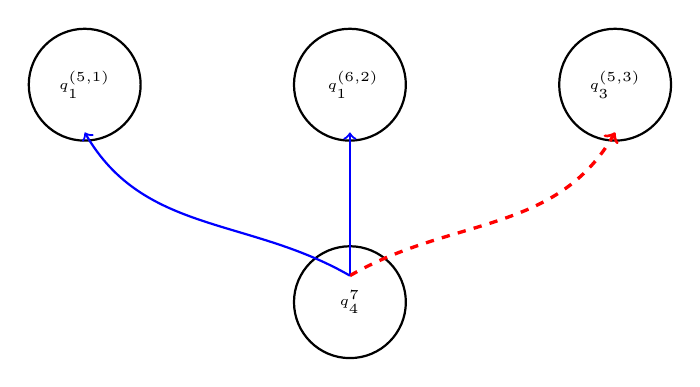
\begin{tikzpicture}[scale=\textwidth/18cm,samples=200]
          %%% The nodes represents the k query in the first round
          % \draw[very thick] (-1,6)  -- (13,6) -- (13,3) -- (-1,3) -- (-1,6);
          % \draw[black] (-2.5, 4) circle (0pt) node [anchor=south]{\textbf{line 4:}};
          \draw[thick] (1, 4.1) circle (30pt) node
          % node[label={above: \small{iteration 1:}}] 
          {\tiny{$q_1^{(5,1)}$}} ;
          \draw[thick] (6, 4.1) circle (30pt) node
          {\tiny{ $q_1^{(6,2)}$}};
           \draw[thick] (11, 4.1) circle (30pt) node 
          {\tiny{$q_3^{(5,3)}$}};
          % \filldraw[black] (-2.5, 0) circle (0pt) node [anchor=south]{\textbf{line 7:}};
          \draw[thick] (6, 0) circle (30pt) node {\tiny{$q_4^7$}};
          \draw[ thick,->, blue] (6, 0.5)  -- (6, 3.2) ;
          \draw[very thick,->, red, dashed] (6, 0.5)  to [out=30,in=240] (11, 3.2) ;
          \draw[ thick,->, blue] (6, 0.5)  to [out=150,in=300]  (1, 3.2) ;
          \end{tikzpicture}
          \caption{}
              \end{centering}
              \end{subfigure}
              \begin{subfigure}{0.5\textwidth}
              \begin{centering}
              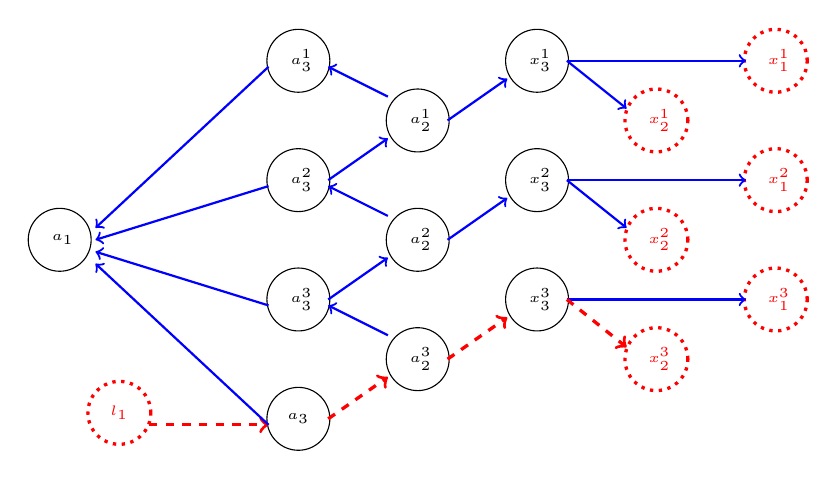
\begin{tikzpicture}[scale=\textwidth/16cm,samples=200]
          %%% The nodes represents the k query in the first round
          % \draw[very thick] (-1,6)  -- (13,6) -- (13,3) -- (-1,3) -- (-1,6);
          % \draw[black] (-2.5, 4) circle (0pt) node [anchor=south]{\textbf{line 4:}};
          % \draw[thick] (1, 1.1) circle (25pt) node
          % % node[label={above: \small{iteration 1:}}] 
          % {\tiny{$q_1^{(5,1)}$}} ;
          \draw[] (2, 5.1) circle (15pt) node
          {\tiny{ $a_1$}};
          \draw[] (6, 8.1) circle (15pt) node
          {\tiny{ $a_3^{1}$}};
          \draw[very thick, red, dotted] (14, 8.1) circle (15pt) node
          {\tiny{ $x_{1}^{1}$}};
          \draw[very thick, red, dotted] (12, 7.1) circle (15pt) node
          {\tiny{ $x_{2}^{1}$}};
          \draw[] (10, 8.1) circle (15pt) node
          {\tiny{ $x_{3}^{1}$}};
          \draw[] (8, 7.1) circle (15pt) node
          {\tiny{ $a_{2}^{1}$}};
          \draw[] (6, 6.1) circle (15pt) node
          {\tiny{ $a_3^{2}$}};
          \draw[very thick, red, dotted] (14, 6.1) circle (15pt) node
          {\tiny{ $x_{1}^{2}$}};
          \draw[very thick, red, dotted] (12, 5.1) circle (15pt) node
          {\tiny{ $x_{2}^{2}$}};
          \draw[] (10, 6.1) circle (15pt) node
          {\tiny{ $x_{3}^{2}$}};
          \draw[] (8, 5.1) circle (15pt) node
          {\tiny{ $a_{2}^{2}$}};
          \draw[very thick, red, dotted] (14, 4.1) circle (15pt) node
          {\tiny{ $x_1^{3}$}};
          \draw[] (6, 4.1) circle (15pt) node
          {\tiny{ $a_3^{3}$}};
          \draw[] (10, 4.1) circle (15pt) node
          {\tiny{ $x_3^{3}$}};
          \draw[very thick, red, dotted] (12, 3.1) circle (15pt) node
          {\tiny{ $x_2^{3}$}};
          \draw[] (8, 3.1) circle (15pt) node
          {\tiny{ $a_{2}^{3}$}};
           \draw[] (6, 2.1) circle (15pt) node 
          {\tiny{$a_3$}};
          % \filldraw[black] (-2.5, 0) circle (0pt) node [anchor=south]{\textbf{line 7:}};
          \draw[very thick, red, dotted] (3, 2.2) circle (15pt) node {\tiny{$l_1$}};
           \draw[very thick,->, red, dashed] (3.5, 2)  -- (5.5, 2) ;
           \draw[very thick,->, red, dashed] (6.5, 2.1)  -- (7.5, 2.8) ;
           \draw[very thick,->, red, dashed] (8.5, 3.1)  -- (9.5, 3.8) ;
           \draw[thick,->, blue] (10.5, 4.1)  -- (13.5, 4.1) ;
            \draw[very thick,->, red, dashed] (10.5, 4.1)  -- (11.5, 3.3) ;
             \draw[thick,->, blue] (7.5, 3.5)  -- (6.5, 4.0) ;
             \draw[thick,->, blue] (6.5, 4.1)  -- (7.5, 4.8) ;
              \draw[thick,->, blue] (8.5, 5.1)  -- (9.5, 5.8) ;
               \draw[thick,->, blue] (10.5, 6.1)  -- (11.5, 5.3) ;
          \draw[thick,->, blue] (10.5, 6.1)  -- (13.5, 6.1) ;
          \draw[thick,->, blue] (7.5, 5.5)  -- (6.5, 6.0) ;
          \draw[thick,->, blue] (6.5, 6.1)  -- (7.5, 6.8) ;
          \draw[thick,->, blue] (8.5, 7.1)  -- (9.5, 7.8) ;
          \draw[thick,->, blue] (10.5, 8.1)  -- (11.5 , 7.3) ;
          \draw[thick,->, blue] (10.5, 8.1)  -- (13.5 , 8.1) ;
          % \draw[thick,->, blue] (8.5, 9.1)  -- (9.5 , 9.8) ;
          % \draw[thick,->, blue] (8, 9.6)  -- (8, 10.6) ;
          \draw[thick,->, blue] (7.5, 7.5)  -- (6.5, 8.0) ;
          \draw[thick,->, blue] (5.5, 8.0)  -- (2.6, 5.3) ;
          \draw[thick,->, blue] (5.5, 6.0)  -- (2.6, 5.1) ;
          \draw[thick,->, blue] (5.5, 4.0)  -- (2.6, 4.9) ;
          \draw[thick,->, blue] (5.5, 2.0)  -- (2.6, 4.7) ;
          % \draw[very thick,->, red] (6, 0.5)  to [out=30,in=240] (11, 3.2) ;
          % \draw[very thick,->, blue] (6, 0.5)  to [out=150,in=300]  (1, 3.2) ;
          \end{tikzpicture}
              \caption{}
              \end{centering}
              \end{subfigure}
              \vspace{-0.3cm}
              \caption{(a) The query-based dependency graph for odd example (b) The SSA variable-based weighted dependency graph for the same example, the node in red dashed circle is weighted.}
              \label{fig:odd_graphs}
              \vspace{-0.3cm}
          \end{figure}